% ============================================================
% SECTION 6 - SIMULATION STUDY
% ============================================================
\section{Simulation Study}
\label{sec:simulations}

The finite-sample behaviour of the schemes is assessed through a
controlled Monte Carlo study in two parts.  The first part takes the
stratified algorithm as the original paper defines it and asks how it
behaves: E1 examines per-season coverage and interval width as a
function of training size, E2 isolates the effect of the per-stratum
sample size $T_s = T/\Sper$, E3 varies the heteroskedasticity intensity
$\sigma_{\mathrm{high}}$, E4 verifies behaviour in the homoskedastic
null, and E5 checks robustness across two base learners.  The second
part asks whether what E1--E5 measure is what it appears to be: E6
compares all eight schemes of Section~\ref{sec:algorithm} across four
seasonal structures, and E7 takes apart the two properties of the
calibration step that make short buffers look worse than they are.
Simulation code is in \texttt{code/simulation.py},
\texttt{code/simulation\_family.py} and
\texttt{code/diag\_linesearch.py}.

%------------------------------------------------------------
\subsection{Experimental Setup}
\label{sec:simulations:setup}
%------------------------------------------------------------

The data-generating process is a seasonal autoregressive model with
heteroskedastic innovations:
\begin{equation}
  \label{eq:dgp_sim}
  Y_t \;=\; 0.6\,Y_{t-12} + 0.3\,Y_{t-1}
       + \sigma_{s(t)}\,\eta_t,
  \qquad
  \eta_t \;\stackrel{\mathrm{iid}}{\sim}\; t_3,
\end{equation}
where $t_3$ denotes the Student $t$-distribution with 3 degrees
of freedom.  The seasonal standard deviations are
\[
  \sigma_s \;=\;
  \begin{cases}
    \sigma_{\mathrm{high}} & \text{if } s \in \{1,2,8,9\}, \\
    1                       & \text{otherwise},
  \end{cases}
\]
with default $\sigma_{\mathrm{high}} = 2$.  The high-volatility
seasons, January, February, August and September, mimic the IPCA
pattern studied in Section~\ref{sec:empirical}, where inflation
surprises are largest at the start of the year and in the pre-harvest
months.  The $t_3$ innovations introduce heavy tails, which makes the
calibration problem harder than it would be under Gaussianity, and
each simulated series begins with a 60-period burn-in that is
discarded.

For each observation at time $t$, the feature vector consists of the
$p = 13$ most recent lags, $x_t = (Y_{t-1}, \ldots, Y_{t-13})$.
The default base learner $\calA$ is Ridge regression
($\ell_2$-penalty $= 1.0$); Experiment E5 also uses a Random Forest
($B_{\mathrm{tree}} = 30$ trees, maximum depth 6).  Both methods use
$B = 50$ bootstrap models, batch size $s_0 = 1$, and significance
level $\alpha = 0.10$.\footnote{Two standard implementation
simplifications are used in the replication code: the test-point
forecast is the simple average of the $B$ bootstrap models rather
than the $\phi$-aggregation of the $T$ LOO predictors (numerically
indistinguishable for $\phi$ = mean), and residuals appended by the
sliding-window update are computed from the full ensemble.
Experiment E5's Random Forest uses $100$ Monte Carlo replications
(all other runs use $n_{\mathrm{rep}} = 200$).  If a SARIMA fit fails
to converge, that replication is scored as non-covered, which, if
anything, penalises the SARIMA benchmark.  All seeds are fixed in the
replication archive.}

Experiments E1--E4 compare three methods:
\begin{enumerate}[label=(\roman*)]
  \item \emph{SARIMA-Gaussian}: a seasonal ARIMA$(1,0,0)(1,0,0)_{12}$
    model fitted by Gaussian maximum likelihood (MLE), with
    symmetric prediction intervals
    $\hat{f}_t \pm z_{1-\alpha/2}\,\hat{\sigma}$,
    where $\hat{\sigma}$ is the in-sample residual standard deviation.
    This is the standard parametric baseline used in applied
    forecasting.
  \item \emph{Pooled EnbPI}: the original algorithm of
    \citet{xu2023conformal}, which maintains a single calibration
    buffer of $T - p$ LOO residuals and uses the distribution-free
    line search of Section~\ref{sec:model:enbpi}.
  \item \emph{\texttt{EnbPI-S}}: Algorithm~\ref{alg:enbpis},
    which maintains $\Sper = 12$ season-specific calibration buffers.
\end{enumerate}
Methods (ii) and (iii) use the same Ridge bootstrap ensemble, so that
the only difference between them lies in calibration, whereas
method (i) differs in both the forecast model (SARIMA against
ensemble) and the interval construction (parametric Gaussian against
empirical quantile).  Experiment E5, on predictor robustness, uses
only methods (ii) and (iii).

Two quantities are recorded for each experiment and each of the
$\Sper = 12$ seasons.  The first is the empirical coverage, the
fraction of $T_1$ test observations in season $s$ whose true value
lies within the predicted interval; the second is the average width,
the mean length of the predicted intervals over test observations in
season $s$.  Overall
(season-averaged) coverage and width are also recorded.  Unless
stated otherwise, $T_1 = 120$ test observations, ten years, are used.
Monte Carlo standard errors are available in the replication archive
(\texttt{code/simulation.py}).

%------------------------------------------------------------
\subsection{E1: Per-Season Coverage and Width}
\label{sec:simulations:e1}
%------------------------------------------------------------

Table~\ref{tab:e1_three_methods_T480} reports per-season empirical
coverage and average width for all three methods at
$T = 480$ (40 years) and $\sigma_{\mathrm{high}} = 2$.
The two-method comparison, Pooled against \texttt{EnbPI-S} only, is
repeated in Appendix~\ref{app:additional}
(Table~\ref{tab:e1_coverage_T480}) as an independent Monte Carlo
replication run with different seeds, so that its entries differ from
those below in the third decimal place.

\begin{table}[ht]
\centering
\small
\caption{Per-season empirical coverage ($90\%$ nominal) for three methods.
$T=480$, $\alpha=0.10$, $S=12$, $n_{\mathrm{rep}}=200$.}
\label{tab:e1_three_methods_T480}
{\setlength{\tabcolsep}{5pt}
\begin{tabular}{l ccc @{\hspace{0.8em}} ccc}
\toprule
 & \multicolumn{3}{c}{Coverage} & \multicolumn{3}{c}{Width} \\
\cmidrule(lr){2-4} \cmidrule(lr){5-7}
Month & SARIMA & Pooled & EnbPI-S & SARIMA & Pooled & EnbPI-S \\
\midrule
Jan* & 0.714 & 0.785 & \textbf{0.829} & 8.06 & \textit{6.38} & 8.20 \\
Feb* & 0.673 & 0.791 & \textbf{0.848} & 8.06 & \textit{6.37} & 8.15 \\
Mar & 0.818 & \textbf{0.955} & 0.845 & 8.06 & 6.38 & \textit{4.27} \\
Apr & \textbf{0.875} & 0.946 & 0.844 & 8.06 & 6.39 & \textit{4.28} \\
May & \textbf{0.899} & 0.947 & 0.842 & 8.06 & 6.39 & \textit{4.25} \\
Jun & \textbf{0.901} & 0.945 & 0.847 & 8.06 & 6.39 & \textit{4.20} \\
Jul & \textbf{0.905} & 0.940 & 0.842 & 8.06 & 6.39 & \textit{4.26} \\
Aug* & 0.744 & 0.795 & \textbf{0.846} & 8.06 & \textit{6.38} & 8.15 \\
Sep* & 0.662 & 0.776 & \textbf{0.844} & 8.06 & \textit{6.37} & 8.25 \\
Oct & 0.782 & \textbf{0.952} & 0.838 & 8.06 & 6.38 & \textit{4.23} \\
Nov & \textbf{0.857} & 0.944 & 0.832 & 8.06 & 6.39 & \textit{4.20} \\
Dec & \textbf{0.883} & 0.938 & 0.833 & 8.06 & 6.39 & \textit{4.19} \\
\bottomrule
\multicolumn{7}{l}{\footnotesize Bold coverage = closest to $90\%$ nominal; italic width = narrowest.  * = high-volatility months ($\sigma_{\mathrm{high}}=2$).} \\
\end{tabular}}
\end{table}

SARIMA$(1,0,0)(1,0,0)_{12}$ is the natural parametric competitor,
since its mean structure closely approximates that of the
DGP~\eqref{eq:dgp_sim}: the multiplicative seasonal AR polynomial
implies an additional cross term $-\phi\Phi\,Y_{t-13} \approx
-0.18\,Y_{t-13}$ that is absent from the additive DGP, though the
two specifications otherwise coincide.  Any material failure in its
prediction intervals is therefore attributable to distributional or
variance misspecification, and not to a poor point forecast, which
makes SARIMA-Gaussian an informative benchmark that isolates the two
ingredients addressed in this paper: non-Gaussianity of the error
distribution ($t_3$ against $\mathcal{N}$) and seasonal
heteroskedasticity of its variance ($\sigma_s \neq \mathrm{const}$).

The pooled method exhibits severe seasonal bias.  Its coverage ranges
from approximately $0.78$ for the high-volatility months (January,
February, August and September, marked with *) to $0.95$ for the
low-volatility months, a range of roughly $0.18$ probability units.
The stratified method compresses this spread to a $0.02$-unit band,
with all twelve months lying between approximately $0.83$ and $0.85$,
which confirms the theoretical prediction of
Proposition~\ref{prop:pooled_gap}: pooled calibration induces a
persistent, season-dependent bias of order $2b_{s^*}$, whereas
stratified calibration removes it.

A complementary view comes from the width column.  The pooled method
produces a nearly constant interval width of $\approx 6.38$ across
all seasons, whereas \texttt{EnbPI-S} widens its intervals by a
factor of $\approx 1.28$ for high-volatility seasons (width
$\approx 8.2$) and narrows them by a factor of $\approx 0.66$ for
low-volatility seasons (width $\approx 4.2$).  The ratio of mean
high-volatility width to mean low-volatility width for
\texttt{EnbPI-S} is approximately $8.2/4.2 \approx 1.95$, closely
tracking the true ratio
$\sigma_{\mathrm{high}}/\sigma_{\mathrm{low}} = 2/1 = 2$, which shows
that \texttt{EnbPI-S} recovers the seasonal volatility structure from
the calibration buffers.

The SARIMA benchmark reveals why a standard parametric approach is
doubly inadequate here.  First, Gaussian prediction intervals
underestimate the heavy tails of the $t_3$ error distribution.
Second, the Gaussian MLE estimates a single $\hat{\sigma}$ from the
pooled residuals, which is relatively too large for the
low-volatility months, whose coverage of $\approx 0.87$ is the
highest SARIMA attains, though still below nominal owing to the
Gaussian tails, and far too small for the high-volatility months,
causing severe undercoverage: mean $0.699$, worst $0.662$ for
September.  The resulting coverage spread of $0.243$ probability
units is $36\%$ wider than that of Pooled EnbPI ($0.179$) and more
than twelve times that of \texttt{EnbPI-S} ($0.019$).  For September
specifically, SARIMA achieves only $66.2\%$ coverage, more than $23$
percentage points below nominal, while \texttt{EnbPI-S} achieves
$84.4\%$.

The comparison isolates the two contributions of the paper.  Pooled
EnbPI corrects SARIMA's distributional assumption through empirical
quantiles, improving high-volatility coverage from $0.699$ to
$0.786$ ($+8.8$ pp); \texttt{EnbPI-S} further corrects the seasonal
calibration bias, raising it to $0.842$ ($+5.5$ pp more) and
collapsing the coverage spread to $0.019$.  Among the three methods,
only \texttt{EnbPI-S} is capable of near-uniform coverage: for the
four high-volatility months (*), SARIMA undercovers by $20$
percentage points on average, Pooled EnbPI by $11$ to $12$
percentage points, and \texttt{EnbPI-S} by $5$ to $7$
percentage points.  September illustrates the contrast starkly, with
SARIMA at $0.662$, Pooled at $0.776$ and \texttt{EnbPI-S} at $0.844$.

From a risk-management perspective the relevant quantity is the
\emph{minimum} per-season coverage.  SARIMA achieves a worst case of
$0.662$ (September) and Pooled EnbPI $0.776$ (September), while
\texttt{EnbPI-S} raises this floor to $0.829$ (January; its September
coverage is $0.844$).  Among these three methods the ordering is
unambiguous, and \texttt{EnbPI-S} provides the strongest guarantee
for the seasons that matter most; Experiment E6 below reopens the
comparison against a fourth scheme.

Table~\ref{tab:e1_coverage_T240} (Appendix~\ref{app:additional})
repeats the analysis for $T = 240$ (20 years).  The qualitative
pattern is identical, with \texttt{EnbPI-S} reducing seasonal
coverage dispersion and narrowing intervals in low-volatility months;
the absolute coverage values are lower for both methods at $T = 240$,
owing to the reduced per-stratum sample size $T_s \approx 20$, a
finite-sample effect studied in Experiment E2 below.

%------------------------------------------------------------
\subsection{E2: Effect of Stratum Size}
\label{sec:simulations:e2}
%------------------------------------------------------------

Theorem~\ref{thm:strat_coverage} predicts that the stratified
coverage bound converges to zero at rate $O(\sqrt{\log T_s / T_s})$,
where $T_s = T/\Sper$ is the per-stratum sample size.
Experiment E2 isolates this effect by varying $T_s \in
\{5, 10, 20, 30, 50\}$, corresponding to $T \in \{60, 120, 240,
360, 600\}$ months, holding $T_1 = 120$ and
$\sigma_{\mathrm{high}} = 2$ fixed.

\begin{table}[ht]
\centering
\caption{Overall empirical coverage and average width vs stratum size $T_s = T/S$.
$\alpha=0.10$, $S=12$, $n_{\mathrm{rep}}=200$.}
\label{tab:e2_stratum_size}
\begin{tabular}{r r cc cc}
\toprule
$T_s$ & $T$ & \multicolumn{2}{c}{Coverage} & \multicolumn{2}{c}{Width} \\
\cmidrule(lr){3-4} \cmidrule(lr){5-6}
& & Pooled & EnbPI-S & Pooled & EnbPI-S \\
\midrule
5 & 60 & 0.836 & 0.516 & 7.423 & 4.132 \\
10 & 120 & 0.865 & 0.701 & 6.632 & 4.932 \\
20 & 240 & 0.879 & 0.785 & 6.457 & 5.295 \\
30 & 360 & 0.890 & 0.822 & 6.417 & 5.452 \\
50 & 600 & 0.887 & 0.845 & 6.387 & 5.631 \\
\bottomrule
\end{tabular}
\end{table}

The results, shown in Table~\ref{tab:e2_stratum_size}, reveal two
phenomena.  First, for very small $T_s$, as in $T_s = 5$,
\texttt{EnbPI-S} falls well short of nominal coverage
($\approx 0.52$), while pooled EnbPI achieves $\approx 0.84$; this is
a genuine finite-sample limitation, since with fewer than ten
residuals per season the per-stratum empirical quantiles are too
noisy to serve as reliable calibration points.  Second, as $T_s$
grows, the stratified coverage improves monotonically from $0.516$ at
$T_s = 5$ to $0.845$ at $T_s = 50$, consistent with the
$O(\sqrt{\log T_s / T_s})$ decay in the theoretical bound.  The
pooled coverage, by contrast, plateaus near $0.88$ once
$T_s \geq 20$ ($0.836$ and $0.865$ at $T_s = 5$ and $10$), since the
persistent bias $2b_{s^*}$ prevents it from converging to the
nominal level.

\begin{remark}[Practical sample-size guidance]
\label{rem:min_ts}
The results suggest that \texttt{EnbPI-S}, \emph{as the original
algorithm builds the interval}, requires at least
$T_s \approx 30$--$40$ observations per season to be competitive
with pooled EnbPI.  For monthly data with $\Sper = 12$, this
corresponds to $T \approx 360$--$480$ months ($30$--$40$ years).
Experiment E6 shows that the requirement is a property of that
construction rather than of stratification, and that it disappears
once the interval is built from conformal order statistics.
The food-IPCA application (Section~\ref{sec:empirical:food})
uses $T = 240$ months ($\Ts = 20$), below this range, which
is consistent with the coverage shortfall observed there.
The export growth application (Section~\ref{sec:empirical:exports})
uses $T = 430$ months ($\Ts \approx 35$), falling within the
recommended range and achieving coverage within $3.3$ percentage
points of nominal.
\end{remark}

%------------------------------------------------------------
\subsection{E3: Heteroskedasticity Intensity}
\label{sec:simulations:e3}
%------------------------------------------------------------

The benefit of stratification grows with the degree of
heteroskedasticity, which Experiment E3 documents by varying
$\sigma_{\mathrm{high}} \in \{1.0, 1.5, 2.0, 3.0\}$ with $T = 240$
fixed.  Table~\ref{tab:e3_intensity} in Appendix~\ref{app:additional}
reports the outcome.

When $\sigma_{\mathrm{high}} = 1$, the null case, identical to E4
below, both methods perform similarly and the advantage of
\texttt{EnbPI-S} is small, limited to coverage uniformity.
As $\sigma_{\mathrm{high}}$ increases, the pooled coverage for
high-volatility seasons deteriorates markedly: at
$\sigma_{\mathrm{high}} = 3$, pooled coverage in January falls to
$\approx 0.70$, while the stratified method maintains coverage near
$0.78$--$0.81$ for the same seasons.  The pooled coverage for
low-volatility months rises at the same time to
$\approx 0.95$--$0.97$, which reflects increasingly inflated
intervals.  \texttt{EnbPI-S} keeps both high- and low-volatility
months near the same, if imperfect, coverage level, and thereby
adapts to an unknown heteroskedasticity intensity.
The width ratio EnbPI-S\,/\,Pooled for high-volatility seasons
tracks $\sigma_{\mathrm{high}}$: at $\sigma_{\mathrm{high}} = 3$,
\texttt{EnbPI-S} produces intervals approximately $1.4\times$ wider
than Pooled for January and February, consistent with the inflated
residual scale for those months.

%------------------------------------------------------------
\subsection{E4: Null Case}
\label{sec:simulations:e4}
%------------------------------------------------------------

To quantify the cost of stratification in the absence of
heteroskedasticity, $\sigma_s = 1$ is imposed for all $s$ with
$T = 240$.  In this case the pooled and stratified buffers are
calibrated on residuals from the same distribution, and the
theoretical bias is $b_{s^*} = 0$.  Table~\ref{tab:e4_null} in
Appendix~\ref{app:additional} reports the per-season detail.

Empirically, pooled EnbPI achieves overall coverage of
$\approx 0.88$, close to the nominal $0.90$, with small variation
across seasons ($\approx 0.87$--$0.89$), whereas \texttt{EnbPI-S}
achieves only $\approx 0.79$ overall, a gap of roughly nine
percentage points.  Under the interval construction of the original
algorithm this gap looks like the \emph{stratification cost}, since
using only $T_s \approx 19$ residuals per season instead of the full
$T - p \approx 227$ enlarges the finite-sample error of the empirical
quantile.  Experiment E6 shows that most of it is not attributable to
stratification at all, and that the same buffer read differently
delivers the nominal level.

The practical implication is direct.  An analyst who is uncertain
whether seasonal heteroskedasticity is present should prefer
\texttt{EnbPI-S} only if there is enough data (see
Remark~\ref{rem:min_ts}) and if the heteroskedasticity is pronounced
enough to outweigh that cost.  The cost falls on stratification and
not on the alternative way of conditioning on the season, since a
seasonally normalised buffer loses only $1.1$ percentage points in
this same null case; Experiment E6 shows why, and that the loss is
avoidable.

%------------------------------------------------------------
\subsection{E5: Predictor Robustness}
\label{sec:simulations:e5}
%------------------------------------------------------------

The seasonal bias identified in Proposition~\ref{prop:pooled_gap}
is a property of the calibration procedure, and not of the point
forecast $\hat{f}$.  Experiment E5 verifies this by repeating the
main experiment with $T = 240$ and $\sigma_{\mathrm{high}} = 2$
under two base learners, Ridge regression and a Random Forest
(Table~\ref{tab:e5_predictor} in Appendix~\ref{app:additional}).
In both cases the qualitative pattern is preserved: pooled EnbPI
overcovers low-volatility seasons and undercovers high-volatility
ones, while \texttt{EnbPI-S} reduces this dispersion.  The magnitude
of the effect is nearly identical across learners, which confirms
that the gain from stratification is \emph{model-agnostic}, since it
depends only on the seasonal structure of the residual distribution
and not on the quality of the point forecast.  The coverage spread
under pooled calibration is $0.183$ with Ridge and $0.179$ with the
Random Forest, against $0.034$ and $0.035$ for \texttt{EnbPI-S}.

%------------------------------------------------------------
\subsection{E6: What the Calibration Step Costs on a Short Buffer}
\label{sec:simulations:e6constr}
%------------------------------------------------------------

The experiments so far attribute every difference between the schemes to
the seasonal structure of the residuals.  Two properties of the
calibration step also punish short buffers, and since the stratified
scheme is the one with short buffers, they are easily mistaken for a cost
of stratification.  Experiment E6 separates them.  It works directly on
residual buffers drawn from a known distribution, without the forecasting
pipeline, so that nothing else can interfere.

The first is the inward bias of extreme empirical quantiles.  Over $1500$
buffers of $\Ts = 20$ residuals drawn from the seasonal scale design of
Section~\ref{sec:simulations:setup}, the empirical $5\%$ and $95\%$
quantiles of a season's own residuals are biased by $+0.28$ and $-0.35$,
that is, inwards at both ends, against a shape discrepancy
$\Delta_{\sstar}$ of $-0.100$ and $+0.047$ at the same two levels.  The
bias exceeds the quantity the calibration is trying to capture by factors
of $2.8$ and $7.4$, and it is a mechanical consequence of the buffer: an
empirical quantile cannot fall outside the range of the sample that
defines it.

That observation has an exact counterpart, and it comes with two
thresholds rather than one.  The conformal prescription is an order
statistic, not a quantile level: the upper endpoint of a two-sided
$1-\alpha$ interval is the $k_{\text{hi}}$-th smallest residual with
$k_{\text{hi}} = \lceil (n+1)(1-\alpha/2)\rceil$ and the lower endpoint
the $k_{\text{lo}}$-th with
$k_{\text{lo}} = \lfloor (n+1)\alpha/2 \rfloor$.  Both indices exist,
so a finite interval exists at all, only when
\begin{equation}
  \label{eq:feasible}
  n \;\geq\; \frac{2}{\alpha} - 1,
\end{equation}
which is $9$, $19$, $39$ and $99$ at $\alpha = 0.20$, $0.10$, $0.05$ and
$0.02$; and both indices fall strictly inside the sample, so that the
endpoints are not the buffer extremes, only when
$n \geq 4/\alpha - 1$, that is $19$, $39$, $79$ and $199$ at the same
four levels.  Between the two thresholds the conformal interval simply is
the range of the buffer, which is valid and conservative but cannot adapt
to anything.  At the $90\%$ level a season buffer needs $19$ observations
for an interval to exist and $39$ before its endpoints move inside the
sample; a monthly series therefore needs $T \geq 228$ months for the first
and $T \geq 468$ for the second.  This is the same limit Experiment E2
located by simulation at $30$ to $40$ observations per season, now with a
reason: it is not about the variance of an estimator but about how many
order statistics a buffer contains.  The two empirical applications of
Section~\ref{sec:empirical} sit at $\Ts = 20$ and $\Ts = 35$, that is
between the thresholds.

\begin{figure}[ht]
  \centering
  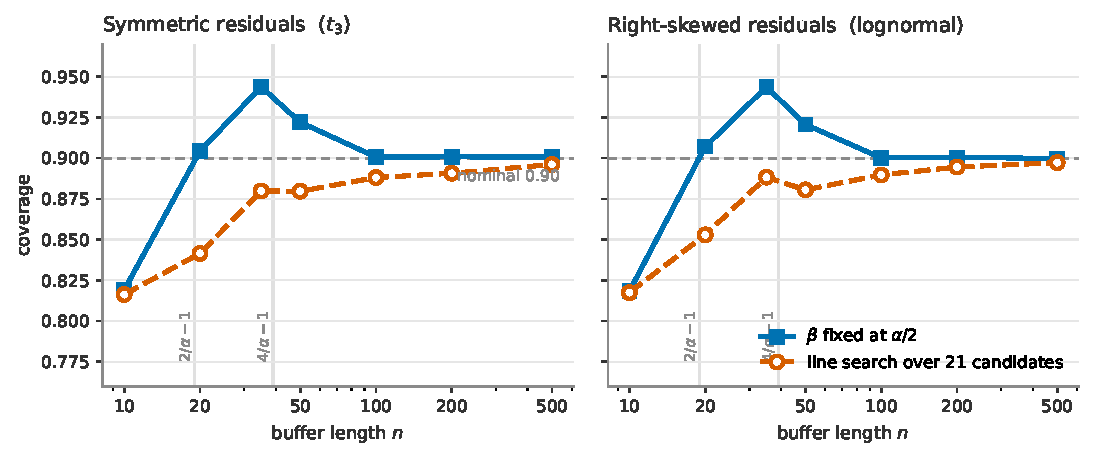
\includegraphics[width=0.95\textwidth]{figures/fig_linesearch_cost}
  \caption{Experiment E6: coverage of a $90\%$ interval built from a
           single buffer of $n$ residuals, with conformal order
           statistics throughout, so that the only difference between
           the two series is whether the asymmetry $\beta$ is fixed at
           $\alpha/2$ or chosen as the narrowest of $21$ candidates
           computed from the same residuals.  The vertical rules are
           the two thresholds of Section~\ref{sec:simulations:e6constr}:
           below the first no finite conformal interval exists, and
           between them the interval is the range of the buffer, which
           is why the fixed-$\beta$ series overshoots there.  With
           $\beta$ fixed the finite-sample guarantee holds at every
           buffer length above the first threshold; the line search
           removes it, by between four and six and a half percentage
           points at the lengths a monthly series provides.  Table~\ref{tab:e9_linesearch} in
           Appendix~\ref{app:additional} adds the widths and a finer
           grid.}
  \label{fig:linesearch_cost}
\end{figure}

The second property is a selection effect in the line search.  The
optimiser returns the narrowest of $m$ candidate quantile pairs, all
computed from the same residuals, and the narrowest of many noisy
candidates is narrower than it ought to be.
Table~\ref{tab:e9_linesearch} measures the consequence with everything
else held fixed, the conformal order statistics being used throughout, so
that the columns differ only in whether $\beta$ is searched.

Read the $m = 1$ column first, because it establishes the benchmark.  With
$\beta$ fixed at $\alpha/2$ and conformal endpoints, coverage is $0.904$
at $n = 20$, $0.922$ at $n = 50$ and $0.901$ at $n = 100$, $200$ and
$500$: the finite-sample guarantee holds, conservatively so between the
two thresholds discussed after~\eqref{eq:feasible}, where the interval is the buffer
range, and tightly once the endpoints move inside.  A season-specific
conformal interval is therefore not intrinsically costly at $\Ts = 20$;
it is exactly as valid as the theory says it is.

The line search voids that.  For symmetric residuals, where the
population-optimal asymmetry is $\beta = \alpha/2$ and the search has
nothing to find, coverage falls from $0.904$ to $0.842$ at $n = 20$, from
$0.922$ to $0.880$ at $n = 50$ and from $0.901$ to $0.896$ at $n = 500$:
between four and six percentage points at the buffer lengths a monthly
series provides, half a point once the buffer is long.  The damage
saturates in $m$, with $21$ candidates doing as much of it as $201$, so
coarsening the grid does not avoid it.  For skewed residuals the search
does find something real, cutting the width by $42\%$ at $n = 20$, from
$3.40$ to $1.96$, but it costs the same five percentage points of
coverage.

The practical conclusion is that the line search is worth running on a
pooled buffer and is not worth running on a season buffer of the length
these data provide.  This matters for how the rest of the paper should be
read: what Sections~\ref{sec:simulations:e2} and~\ref{sec:simulations:e4}
report as the cost of stratification is in large part the cost of
combining stratification with a quantile estimator that carries no
finite-sample guarantee and with a selection step that removes what
guarantee remains.  Conditioning the calibration on the season is cheap;
the way EnbPI turns a buffer into an interval is what is expensive when
the buffer is short.

\begin{remark}[On scoring interval methods]
\label{rem:winkler}
It is tempting to settle these comparisons with a proper scoring rule, and
the interval score of \citet{winkler1972decision} is the natural
candidate.  It is not neutral here.  Writing
$S(l,u;y) = (u-l) + \tfrac{2}{\alpha}[(l-y)\Ind{y<l} + (y-u)\Ind{y>u}]$,
its expectation satisfies $\partial \E[S]/\partial l = -1 +
\tfrac{2}{\alpha}F(l)$ and $\partial \E[S]/\partial u = 1 -
\tfrac{2}{\alpha}(1-F(u))$, so it is minimised at
$l = F^{-1}(\alpha/2)$ and $u = F^{-1}(1-\alpha/2)$: the score is proper
for the \emph{central} interval, whereas the line search targets the
\emph{narrowest} interval of nominal coverage.  The two functionals differ
whenever the residual distribution is skewed, and the score then favours a
fixed $\beta = \alpha/2$ by construction rather than on merit.  We
therefore report coverage and width as the primary quantities throughout
and use the score only to compare schemes that target the same functional.
\end{remark}

%------------------------------------------------------------
\subsection{E7: Which Scheme, and How the Interval Is Built}
\label{sec:simulations:e7schemes}
%------------------------------------------------------------

Experiment E6 puts the two ways of conditioning on the season, and the
two repairs of Section~\ref{sec:algorithm:defects}, in the same design.
Eight schemes are compared: pooled, normalised and stratified
calibration exactly as the original algorithm builds them, each of the
three again with the conformal order statistics and $\beta$ fixed at
$\alpha/2$ (marked with a dagger), and two members of the interior of the
family, one with the weight fixed at one half and one with the weight
chosen per season by cross-validated coverage on the training buffer.
Within a replication all eight share the same bootstrap ensemble and the
same residuals, so nothing but the calibration step separates them.

Four data-generating processes are used, all with the autoregressive
structure of~\eqref{eq:dgp_sim} and differing only in how the seasons
differ.  In the first the seasons differ in scale alone, as in
Assumption~\ref{ass:seasonal}, with $\sigma_{\mathrm{high}} = 2$.  In the
second they differ in shape alone: every season has unit innovation
variance and the four seasons $\{1,2,8,9\}$ draw a standardised
lognormal innovation, strongly right-skewed, against a standard normal
elsewhere.  The third combines the two.  The fourth is the homoskedastic
null, in which the seasons do not differ at all.  Together they cover the
cases in which each scheme is correctly specified and the cases in which
it is not.

\begin{table}[ht]
\centering
\small
\setlength{\tabcolsep}{4pt}
\caption{Experiment E6: calibration schemes across four
         data-generating processes at $\Ts = 20$
         ($\alpha = 0.10$, $n_{\mathrm{rep}} = 200$; Monte Carlo
         standard errors of the coverage entries do not exceed
         $0.0035$).  A dagger marks the two
         repairs of Section~\ref{sec:algorithm:defects}: conformal
         order statistics and $\beta$ fixed at $\alpha/2$.  Spread
         is the largest minus the smallest per-season coverage,
         Worst the smallest.  All schemes share one ensemble per
         replication.}
\label{tab:e6_schemes}
\begin{tabular}{l cccc cccc}
\toprule
 & \multicolumn{4}{c}{Coverage} & \multicolumn{4}{c}{Spread} \\
\cmidrule(lr){2-5}\cmidrule(lr){6-9}
Method & Scale & Shape & Both & None & Scale & Shape & Both & None \\
\midrule
Pooled & 0.880 & 0.882 & 0.882 & 0.882 & 0.181 & 0.099 & 0.040 & 0.016 \\
\texttt{EnbPI-N} & 0.862 & 0.867 & 0.868 & 0.866 & 0.021 & 0.098 & 0.105 & 0.019 \\
\texttt{EnbPI-S} & 0.785 & 0.790 & 0.790 & 0.789 & 0.032 & 0.036 & 0.042 & 0.027 \\
\midrule
Pooled$^\dagger$ & 0.903 & 0.903 & 0.902 & 0.903 & 0.155 & 0.083 & 0.058 & 0.011 \\
\texttt{EnbPI-N}$^\dagger$ & 0.885 & 0.888 & 0.890 & 0.890 & 0.027 & 0.111 & 0.116 & 0.018 \\
\texttt{EnbPI-S}$^\dagger$ & 0.898 & 0.900 & 0.898 & 0.901 & 0.029 & 0.021 & 0.027 & 0.021 \\
\texttt{EnbPI-H}($\hat\lambda$) & 0.903 & 0.908 & 0.908 & 0.904 & 0.024 & 0.029 & 0.033 & 0.016 \\
\texttt{EnbPI-H}($\tfrac12$) & 0.908 & 0.913 & 0.914 & 0.909 & 0.018 & 0.053 & 0.058 & 0.015 \\
\bottomrule
\multicolumn{9}{l}{\footnotesize Nominal coverage $0.90$.  Column headings name the seasonal structure of the errors: scale only,}\\
\multicolumn{9}{l}{\footnotesize shape only, both, or none.}\\
\end{tabular}
\end{table}


Table~\ref{tab:e6_schemes} reports the hardest sample size,
$\Ts = 20$, which is the food-IPCA application of
Section~\ref{sec:empirical:food}.  Three things stand out.

The first is that the seasonal question is settled as the theory says it
should be.  Pooled calibration leaves a coverage spread of $0.181$ when
the seasons differ in scale, and normalisation removes it, cutting the
spread to $0.021$; but when the seasons differ in shape, normalisation
leaves $0.098$, no better than the $0.099$ of pooling, while
stratification cuts it to $0.036$.  Stratification is the only one of the
two that produces a small spread in all four designs, which is what
Section~\ref{sec:algorithm:normalised} predicts: normalisation is
correctly specified exactly when Assumption~\ref{ass:seasonal} holds, and
that assumption is a modelling choice rather than a fact.

The second is larger, and it concerns the coverage level rather than its
uniformity.  Stratified calibration as the original algorithm builds it
covers $0.785$, $0.790$, $0.790$ and $0.789$ in the four designs, eleven
percentage points below nominal, which is the finding that the earlier
sections of this paper, and the guidance in the literature, read as the
price of conditioning on the season.  The same buffer, read with
conformal order statistics and a fixed $\beta$, covers $0.898$, $0.900$,
$0.898$ and $0.901$.  The eleven points were not the price of
conditioning; they were the price of two choices in how a buffer is
turned into an interval, and Experiment E6 takes each of them apart.
Note that the repair helps pooled and normalised calibration too, by
about two percentage points, but there it is a detail: on a buffer of
$T - p \approx 227$ residuals neither defect bites.

The third is that the interior of the family earns its place on width
rather than on coverage.  At $\Ts = 20$ the daggered stratified scheme
attains its nominal level, but between the two thresholds
of~\eqref{eq:feasible} its endpoints are the extremes of the season
buffer, so it is wide: $9.22$ against $6.46$ for pooled calibration in
the scale design.  Blending it with the normalised endpoint at
$\lambda = \tfrac12$ keeps coverage at $0.908$ and brings the width down
to $8.24$, an eleven per cent reduction, and the cross-validated weight
behaves similarly.  Table~\ref{tab:e6_ts} follows the same schemes as
$\Ts$ grows and shows where the width goes.

\begin{table}[ht]
\centering
\small
\setlength{\tabcolsep}{4pt}
\caption{Experiment E6, continued: coverage and mean width as the
         per-stratum size grows, under seasonal scale
         heterogeneity ($n_{\mathrm{rep}} = 200$).  The
         non-monotonicity of the daggered schemes is the
         discreteness of the conformal index: at $\Ts = 20$ and
         $35$ the endpoints are the buffer extremes, at $\Ts = 50$
         they move inside.}
\label{tab:e6_ts}
\begin{tabular}{l cc cc cc}
\toprule
 & \multicolumn{2}{c}{$\Ts = 20$} & \multicolumn{2}{c}{$\Ts = 35$} & \multicolumn{2}{c}{$\Ts = 50$} \\
\cmidrule(lr){2-3}\cmidrule(lr){4-5}\cmidrule(lr){6-7}
Method & Coverage & Width & Coverage & Width & Coverage & Width \\
\midrule
\texttt{EnbPI-S} & 0.785 & 5.30 & 0.832 & 5.52 & 0.846 & 5.64 \\
\texttt{EnbPI-S}$^\dagger$ & 0.898 & 9.22 & 0.944 & 11.28 & 0.919 & 8.15 \\
\texttt{EnbPI-H}($\tfrac12$) & 0.908 & 8.24 & 0.934 & 9.01 & 0.913 & 7.37 \\
\texttt{EnbPI-H}($\hat\lambda$) & 0.903 & 9.18 & 0.932 & 9.34 & 0.909 & 7.29 \\
Pooled & 0.880 & 6.46 & 0.891 & 6.40 & 0.888 & 6.40 \\
\texttt{EnbPI-N}$^\dagger$ & 0.885 & 7.26 & 0.896 & 6.74 & 0.893 & 6.59 \\
\bottomrule
\multicolumn{7}{l}{\footnotesize Nominal coverage $0.90$.}\\
\end{tabular}
\end{table}


The non-monotonicity in that table is worth a word, because it is
structural rather than noise.  At $\Ts = 20$ and $\Ts = 35$ the
conformal indices sit at the ends of the season buffer, so the interval
is the buffer range and grows with the buffer, which is why coverage
rises from $0.898$ to $0.944$ and the width from $9.22$ to $11.28$.  At
$\Ts = 50$ the indices move inside, the interval stops being the range,
and both fall back, to $0.919$ and $8.15$.  A practitioner reading
Table~\ref{tab:e6_ts} should not conclude that more data hurts; the
conservatism between the thresholds is the price of a finite-sample
guarantee on a short buffer, and the blend is what buys part of it back.

Two things this experiment does not show are worth stating as plainly as
the ones it does.  The first is that the cross-validated weight does not
beat a fixed one half.  Across the twelve cells its coverage is never
more than $0.6$ percentage points away, always on the low side, and its
interval is narrower in only four of them, by at most $1.2$ per cent,
while being up to eleven per cent wider in the others.  What it does buy is
seasonal uniformity, and only where the seasons differ in shape: at
$\Ts = 20$ its spread is $0.029$ against $0.053$ under shape
heterogeneity and $0.033$ against $0.058$ under both, with no advantage
in the other two designs.  Choosing the weight from data is therefore
defensible but not important; the repairs are what matter.

The second is that no season-conditional scheme reaches the nominal
level at $\Ts = 20$ while staying as narrow as the schemes that ignore
the season.  Pooled calibration with the repair covers $0.903$ at a width
of $7.11$, against $9.22$ for the stratified version, and it does so
while leaving a coverage spread of $0.155$: it is narrow because it is
wrong in the direction the paper is about.  At twenty observations per
season the choice is between a valid wide interval and a narrow one with
no season-conditional guarantee, and that is a statement about what
twenty observations can support rather than about any algorithm.

%------------------------------------------------------------
\subsection{Summary}
\label{sec:simulations:summary}
%------------------------------------------------------------

Table~\ref{tab:sim_summary} below summarises the key
trade-offs across experiments.

\begin{table}[ht]
\centering
\caption{Summary of simulation findings.
         \cmark\ = advantage, \xmark\ = disadvantage,
         $\approx$ = comparable.  \texttt{EnbPI-N} is the
         seasonally normalised scheme of Experiment E6.}
\label{tab:sim_summary}
\begin{tabular}{l cccc}
\toprule
Criterion & SARIMA & Pooled & \texttt{EnbPI-N}$^\dagger$ & \texttt{EnbPI-S}$^\dagger$ \\
\midrule
Distribution-free interval shape          & \xmark & \cmark & \cmark & \cmark \\
Coverage uniformity, scale heterogeneity  & \xmark & \xmark & \cmark & \cmark \\
Coverage uniformity, shape heterogeneity  & \xmark & \xmark & \xmark & \cmark \\
Width adaptation across seasons           & \xmark & \xmark & \cmark & \cmark \\
Worst-case per-season coverage            & \xmark & \xmark & $\approx$ & \cmark \\
Overall coverage level at $\Ts = 20$      & \xmark & \cmark & \cmark & \cmark \\
Interval width at $\Ts = 20$              & \cmark & \cmark & $\approx$ & \xmark \\
Free of a seasonal scale model            & \xmark & \cmark & \xmark & \cmark \\
Robustness to predictor choice            & -- & \cmark & -- & \cmark \\
\bottomrule
\end{tabular}
\end{table}

The comparison with the parametric benchmark tells a progressive story.
SARIMA-Gaussian fails on both axes, since it underestimates heavy tails
and ignores seasonal variance differences, producing a worst-case
coverage of $0.662$ in September
(Table~\ref{tab:e1_three_methods_T480}).  Pooled EnbPI corrects the
distributional assumption through empirical quantiles, improving
worst-case coverage to $0.776$, though it retains the seasonal bias of
pooled calibration.  Stratified calibration corrects both, and with the
repairs of Section~\ref{sec:algorithm:defects} it does so without paying
the coverage penalty that Experiments E2 and E4 report.

The summary of the whole study is therefore in two parts.  On the
seasonal question, both ways of conditioning on the season remove the
bias of Proposition~\ref{prop:pooled_gap} when the season enters through
the scale, and only stratification removes it when the season enters
through the shape; since which of the two holds is a modelling
assumption rather than an observable, stratification is the conservative
choice, and Section~\ref{sec:empirical} shows how to test the assumption
on data.  On the finite-sample question, what E2 and E4 measure as the
cost of stratification is almost entirely the cost of two choices in the
calibration step: with conformal order statistics and a fixed asymmetry,
a season buffer of twenty residuals delivers its nominal level in all
four seasonal structures.  What remains is a cost in width, not in
coverage, and it is the honest price of a finite-sample guarantee on a
short buffer; blending the two endpoints recovers about a tenth of it.
